\documentclass[tikz,border=8pt]{standalone}
% Shared look for every TikZ diagram. Load with \input{../../tools/tikz-style.tex}
\usepackage[T1]{fontenc}
\usepackage{lmodern}
\renewcommand{\sfdefault}{lmr}  % diagrams use the same serif as the text
\usetikzlibrary{arrows.meta, positioning, shapes.geometric, calc, fit, backgrounds}
\definecolor{cblue}{HTML}{4C78A8}
\definecolor{corange}{HTML}{F58518}
\definecolor{cgreen}{HTML}{54A24B}
\definecolor{cred}{HTML}{E45756}
\definecolor{cpurple}{HTML}{B279A2}
\definecolor{cgrey}{HTML}{6B6B6B}
\tikzset{
  every picture/.style={font=\sffamily, line width=1.2pt},
  box/.style={draw=#1, fill=#1!12, rounded corners=4pt, align=center, inner sep=7pt, minimum height=1.1cm},
  box/.default=cgrey,
  arrow/.style={-{Stealth[length=3mm]}, draw=cgrey, line width=1.4pt},
  title/.style={font=\sffamily\bfseries\Large},
  note/.style={font=\sffamily\small, text=cgrey, align=center},
}
\AtBeginDocument{\hyphenpenalty=10000 \exhyphenpenalty=10000}

\begin{document}
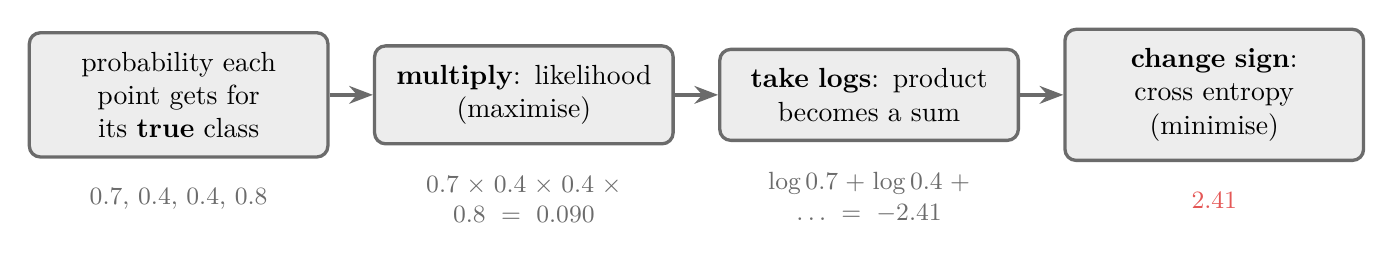
\begin{tikzpicture}[node distance=0.55cm]
  \node[box, text width=3.3cm] (a) {probability each point gets for its \textbf{true} class};
  \node[box, text width=3.3cm, right=of a] (b) {\textbf{multiply}: likelihood\\(maximise)};
  \node[box, text width=3.3cm, right=of b] (c) {\textbf{take logs}: product becomes a sum};
  \node[box, text width=3.3cm, right=of c] (d) {\textbf{change sign}: cross entropy\\(minimise)};
  \draw[arrow] (a) -- (b); \draw[arrow] (b) -- (c); \draw[arrow] (c) -- (d);
  \node[note, below=0.25cm of a, text width=3.3cm] {0.7, 0.4, 0.4, 0.8};
  \node[note, below=0.25cm of b, text width=3.3cm] {$0.7 \times 0.4 \times 0.4 \times 0.8 = 0.090$};
  \node[note, below=0.25cm of c, text width=3.3cm] {$\log 0.7 + \log 0.4 + \dots = -2.41$};
  \node[note, below=0.25cm of d, text width=3.3cm, text=cred] {$2.41$};
\end{tikzpicture}
\end{document}
